\documentclass{beamer}
\usepackage[utf8]{inputenc}

\title{JEE problem}
\author{C.Sriram Saran-EE18BTECH11007 &Krupateja-EE18BTECH11015}

\date{14 February 2019}
\usepackage{natbib}
\usepackage{graphicx}

\begin{document}

\maketitle

\begin{frame}{Question}
A circle C of radius 1 is inscribed in an equilateral triangle PQR. The points of contact of C with the sides PQ, QR, RP are D, E, F, respectively. The line PQ is given by the equation
\sqrt{3}x +y-6=0 \\the point D is (3\sqrt{3}/2,3/2)\\
Further, it is given that the origin and the centre of C are on the same side of the line PQ.\\
Q.18. The equation of circle C is?
\end{frame}


\begin{frame}{Solution}
The centre of the circle will lie on the normal to line PQ\\
D=\begin{bmatrix}
3\sqrt{3}/2\\
 3/2
\end{bmatrix} \\
PQ= \begin{bmatrix}
1\\
-\sqrt{3}
\end{bmatrix} is direction vector of PQ\\
omat=\begin{bmatrix}
0&1\\
-1&0
\end{bmatrix}. 


direction of normal to PQ is\\
N1 = \begin{bmatrix}
0&1\\
-1&0
\end{bmatrix}\times \begin{bmatrix}
-1\\
\sqrt{3}
\end{bmatrix}=\begin{bmatrix}
\sqrt{3}\\
1
\end{bmatrix}\\
centre C lies on C= D+K\times N1\\
here norm(C-D)=1 \\
K is obtained  as 1/norm(N1)\
i.e K=1/2 \\
so C is \begin{bmatrix}
\sqrt{3}\\
1\\
\end{bmatrix}\\
equation of circle is obtained as (norm(X-C))^2=1\\
(X-C)(X-C)^T=1
Where X=\begin{bmatrix}
x\\
y
\end{bmatrix}\\

\end{frame}

\begin{frame}

Q19-Find points E and F -\\
Solution-\\
P =D +K\times PQ\\
norm(P-D)=\sqrt{3}\\
K=\sqrt{3}/norm(PQ)=\sqrt{3}/2\\
P=\begin{bmatrix}
2\sqrt{3}\\
0
\end{bmatrix}\\
since D is mid point of PQ \\
Q=2D-P\\

M= \begin{bmatrix}
cos(i) & -sin(i)\\
sin(i) & cos(i) 
\end{bmatrix}\\
i=\pi/3\\
Multiply M with PQ to obtain Direction of RQ\\
\begin{equation}
x=\begin{bmatrix}
cos(i)&-sin(i)\\
sin(i)&cos(i)
\end{bmatrix}^T\begin{bmatrix}
-1\\
+\sqrt{3}
\end{bmatrix}
\end{equation}
\therefore  RQ=\begin{bmatrix}
1\\
\sqrt{3}
\end{bmatrix}




\end{frame}
\begin{frame}
R-Q=K\times RQ\\
norm(R-Q)=2\sqrt{3}
K=2\sqrt{3}/norm(RQ)=\sqrt{3}\\
R=\begin{bmatrix}
0\\
0\\

\end{bmatrix}\\
E=(Q+R)/2,F=(R+P)/2 \\
\end{frame}

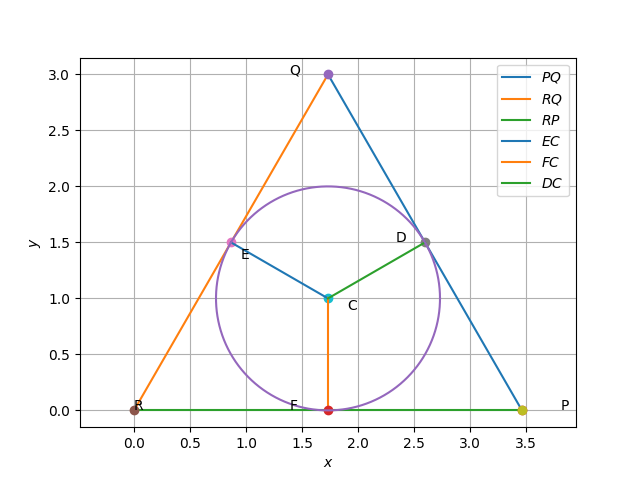
\includegraphics[width=\textwidth]{preambule/EE1390PROJECT.png}}


\end{document}

